%%%%%%%%%%%%%%%%%%%%%%%%%%%%%%%%%%%%
% 配布用ハンドアウト（解答なし）
% コンパイルコマンド: lualatex chp6_handout.tex
%%%%%%%%%%%%%%%%%%%%%%%%%%%%%%%%%%%%

\documentclass[slidestop,compress,mathserif,handout]{beamer}

% 解答を非表示にする
\newcommand{\soln}[1]{ }
\newcommand{\solnGr}[1]{ }

% 4スライドを1ページに印刷する設定
\usepackage{pgfpages}
\pgfpagesuselayout{4 on 1}[a4paper,landscape,border shrink=5mm]

%%%%%%%%%%%%%%%%%%%%%%%%%%%%%%%%%%%%
% 日本語サポート（LuaLaTeX使用）
%%%%%%%%%%%%%%%%%%%%%%%%%%%%%%%%%%%%

\usepackage{luatexja}
\usepackage{luatexja-fontspec}

%%%%%%%%%%%%%%%%%%%%%%%%%%%%%%%%%%%%
% スタイル
%%%%%%%%%%%%%%%%%%%%%%%%%%%%%%%%%%%%

\input{../lec_style_JP}

% 配布用：練習問題の正解を通常アイテムとして表示（オーバーレイなし）
\renewcommand{\solnMult}[1]{\item #1}

\setbeamertemplate{footline}{%
  \insertframenumber\,/\,\inserttotalframenumber}

%%%%%%%%%%%%%%%%%%%%%%%%%%%%%%%%%%%%
% プリアンブル
%%%%%%%%%%%%%%%%%%%%%%%%%%%%%%%%%%%%

\title[第6章：カテゴリデータの推測]{第6章：カテゴリデータの推測}
\author{OpenIntro Statistics 第4版（日本語版）}
\institute{$\:$ \\ {\footnotesize 原著スライド：Mine \c{C}etinkaya-Rundel（OpenIntro）\\
\webLink{http://creativecommons.org/licenses/by-sa/3.0/us/}{CC BY-SA ライセンス}のもと使用・翻訳。\\
一部の画像はフェアユース（教育目的）に基づき使用。}}
\date{}

%%%%%%%%%%%%%%%%%%%%%%%%%%%%%%%%%%%%
% ドキュメント開始
%%%%%%%%%%%%%%%%%%%%%%%%%%%%%%%%%%%%

\begin{document}


%%%%%%%%%%%%%%%%%%%%%%%%%%%%%%%%%%%%
% タイトルページ
%%%%%%%%%%%%%%%%%%%%%%%%%%%%%%%%%%%%

{
\addtocounter{framenumber}{-1}
{\removepagenumbers
\usebackgroundtemplate{
\includegraphics[width=\paperwidth]{../OpenIntro_Grid_4_3-01.jpg}}
\begin{frame}

\hfill 
\includegraphics[width=20mm]{../oiLogo_highres}

\titlepage

\end{frame}
}
}


%%%%%%%%%%%%%%%%%%%%%%%%%%%%%%%%%%%%
% 各節
%%%%%%%%%%%%%%%%%%%%%%%%%%%%%%%%%%%%

%%%%%%%%%%%%%%%%%%%%%%%%%%%%%%%%%%%%

\section{単一割合の推測}

%%%%%%%%%%%%%%%%%%%%%%%%%%%%%%%%%%%%

\begin{frame}

\pq{2人の科学者が、ある薬が高血圧に有効かどうかを調べたいと考えています。1人目の科学者は、高血圧を持つ1000人にその薬を投与し、血圧が下がった人数を記録しようとしています。2人目の科学者は、高血圧を持つ500人に薬を投与し、別の高血圧を持つ500人には投与しないで、両グループで血圧が下がった人数を比較しようとしています。この薬を試験するためにより良い方法はどちらですか？}

\begin{enumerate}[(a)]
\item 1000人全員に薬を投与する
\solnMult{500人に投与し、500人には投与しない}
\end{enumerate}

\end{frame}

%%%%%%%%%%%%%%%%%%%%%%%%%%%%%%%%%%%%

\begin{frame}
\frametitle{GSSの結果}

GSSは同じ質問を行っており、以下は2010年の調査の回答の分布です：\\

\begin{center}
\begin{tabular}{l c}
1000人全員に薬を投与する		& 99 \\
500人に投与し、500人には投与しない	& 571 \\
\hline
合計					& 670
\end{tabular}
\end{center}

\end{frame}

%%%%%%%%%%%%%%%%%%%%%%%%%%%%%%%%%%%

\begin{frame}
\frametitle{母数（パラメータ）と点推定値}

\dq{実験計画について正しい直感を持つ、つまり「500人に投与し、500人には投与しない」と答えるアメリカ人全体の割合を推定したいと思います。関心のある母数（パラメータ）と点推定値は何ですか？}

\begin{itemize}

\item \hl{関心のある母数（パラメータ）：}\orange{全}アメリカ人のうち、実験計画について正しい直感を持つ人の割合。
\[ \mathhl{p}~\scriptsize{(\text{母集団の割合})} \]

\item \hl{点推定値：}\orange{標本抽出された}アメリカ人のうち、実験計画について正しい直感を持つ人の割合。
\[ \mathhl{\hat{p}}~\scriptsize{(\text{標本の割合})} \]

\end{itemize}

\end{frame}

%%%%%%%%%%%%%%%%%%%%%%%%%%%%%%%%%%%

\begin{frame}
\frametitle{割合の推測}

\dq{実験計画について正しい直感を持つ、つまり「500人に投与し、500人には投与しない」と答えるアメリカ人全体の割合は何パーセントですか？}

\begin{itemize}

\item この研究上の問いは信頼区間を使って答えることができます。信頼区間は常に次の形をとります：

\[ \textcolor{orange}{点推定値 \pm 誤差の範囲} \]

\item また、\textcolor{orange}{$誤差の範囲 = 臨界値 \times 点推定値の標準誤差$}であることも知っています。

\end{itemize}

\formula{標本割合の標準誤差}
{
\[ SE_{\hat{p}} =  \sqrt{\frac{p~(1-p)}{n}}  \]
}


\end{frame}

%%%%%%%%%%%%%%%%%%%%%%%%%%%%%%%%%%%

\subsection{標本割合がほぼ正規分布に従う場合の確認}

%%%%%%%%%%%%%%%%%%%%%%%%%%%%%%%%%%%%

\begin{frame}
\frametitle{標本割合もほぼ正規分布に従う}

\formula{割合の中心極限定理}
{
標本割合は、母集団の割合$p$を平均とし、標準誤差$\sqrt{\frac{p~(1-p)}{n}}$を持つ正規分布にほぼ従います。
\[ \hat{p} \sim N \pr{ mean = p, SE = \sqrt{\frac{p~(1-p)}{n}} } \]
}

もちろん、これはある条件のもとでのみ成り立ちます…

\dq{何か予想できますか？}

\soln{独立な観測値、少なくとも10の成功と10の失敗}

\Note{$p$が未知の場合（ほとんどのケース）、標準誤差の計算に$\hat{p}$を使用します。}

\end{frame}

%%%%%%%%%%%%%%%%%%%%%%%%%%%%%%%%%%%

\subsection{割合の信頼区間}

%%%%%%%%%%%%%%%%%%%%%%%%%%%%%%%%%%%%

\begin{frame}
\frametitle{実験計画の話に戻ろう…}

\dq{GSSによると、670人中571人（85\%）のアメリカ人が実験計画に関する質問に正しく回答しました。実験計画について正しい直感を持つアメリカ人全体の割合を、95\%信頼区間を用いて推定してください。}

与えられた値：$n = 670, \hat{p} = 0.85$。まず条件を確認します。

\begin{enumerate}[1.]
\item \hl{独立性：}標本は無作為に抽出されており、670 $<$ 全アメリカ人の10\%であるため、ある回答者の回答が別の回答者の回答と独立していると仮定できます。
\item \hl{成功・失敗条件：}571人が正しく回答（成功）し、99人が誤って回答（失敗）しており、両方とも10以上です。
\end{enumerate}

\end{frame}

%%%%%%%%%%%%%%%%%%%%%%%%%%%%%%%%%%%

\begin{frame}

\pq{$n = 670, \hat{p} = 0.85$が与えられており、標本割合の標準誤差は$SE = \sqrt{\frac{p(1-p)}{n}}$であることを学びました。95\%信頼区間の正しい計算式はどれですか？}

\begin{enumerate}[(a)]
\solnMult{$0.85 \pm 1.96 \times \sqrt{\frac{0.85 \times 0.15}{670}}$} \only<2->{\orange{$\rightarrow (0.82, 0.88)$}}
\item $0.85 \pm 1.65 \times \sqrt{\frac{0.85 \times 0.15}{670}}$
\item $0.85 \pm 1.96 \times \frac{0.85 \times 0.15}{\sqrt{670}}$
\item $571 \pm 1.96 \times \sqrt{\frac{571 \times 99}{670}}$
\end{enumerate}

\end{frame}

%%%%%%%%%%%%%%%%%%%%%%%%%%%%%%%%%%

%%%%%%%%%%%%%%%%%%%%%%%%%%%%%%%%%%%

\subsection{割合を推定する際の標本サイズの選択}

%%%%%%%%%%%%%%%%%%%%%%%%%%%%%%%%%%%

\begin{frame}
\frametitle{標本サイズの選択}

\dq{95\%信頼区間の誤差の範囲を1\%に抑えるためには、何人を標本抽出する必要がありますか？}
\[ ME = z^\star \times SE\]
\begin{eqnarray*}
0.01 &\ge& 1.96 \times \sqrt{\frac{0.85 \times 0.15}{n}} \orange{$\rightarrow$ \text{前の研究の$\hat{p}$を使用}} \\
0.01^2 &\ge& 1.96^2 \times \frac{0.85 \times 0.15}{n} \\
n &\ge& \frac{1.96^2 \times 0.85 \times 0.15}{0.01^2} \\
n &\ge& 4898.04 \orange{~$\rightarrow$ nは少なくとも4,899必要}
\end{eqnarray*}

\end{frame}

%%%%%%%%%%%%%%%%%%%%%%%%%%%%%%%%%%%

\begin{frame}
\frametitle{過去の研究がない場合は？}

… $\hat{p} = 0.5$を使用します

\vspace{1cm}

\dq{なぜですか？}

\begin{itemize}
\item 何もわからない場合、50-50が最も合理的な推測です
\item $\hat{p} = 0.5$は最も保守的な推定値を与えます — 最大の標本サイズが必要
\end{itemize}

\end{frame}

%%%%%%%%%%%%%%%%%%%%%%%%%%%%%%%%%%%%

\subsection{割合の仮説検定}

%%%%%%%%%%%%%%%%%%%%%%%%%%%%%%%%%%%%%

\begin{frame}
\frametitle{割合のCIとHT}

\begin{itemize}

\item 成功・失敗条件：
\begin{itemize}
\item CI：少なくとも10の\orange{観測された}成功と失敗
\item HT：帰無値を使って計算した、少なくとも10の\orange{期待される}成功と失敗
\end{itemize}

\item 標準誤差：
\begin{itemize}
\item CI：観測された標本割合を使って計算：$SE = \sqrt{\frac{\hat{p}(1-\hat{p})}{n}}$
\item HT：帰無値を使って計算：$SE = \sqrt{\frac{p_0(1-p_0)}{n}}$
\end{itemize}

\end{itemize}

\end{frame}

%%%%%%%%%%%%%%%%%%%%%%%%%%%%%%%%%%%

\begin{frame}
\frametitle{}

\dq{GSSによると、670人中571人（85\%）のアメリカ人が実験計画に関する質問に正しく回答しました。このデータは、80\%以上のアメリカ人が実験計画について正しい直感を持つという説得力のある証拠を提供しますか？}

\[ H_0: p = 0.80 \qquad H_A: p > 0.80 \]

\twocol{0.6}{0.4}
{
\begin{eqnarray*}
SE &=& \sqrt{\frac{0.80 \times 0.20}{670}} = 0.0154 \\
Z &=& \frac{0.85 - 0.80}{0.0154} = 3.25 \\
p\text{値} &=& 1 - 0.9994 = 0.0006 \\
\end{eqnarray*}
}
{
\begin{center}
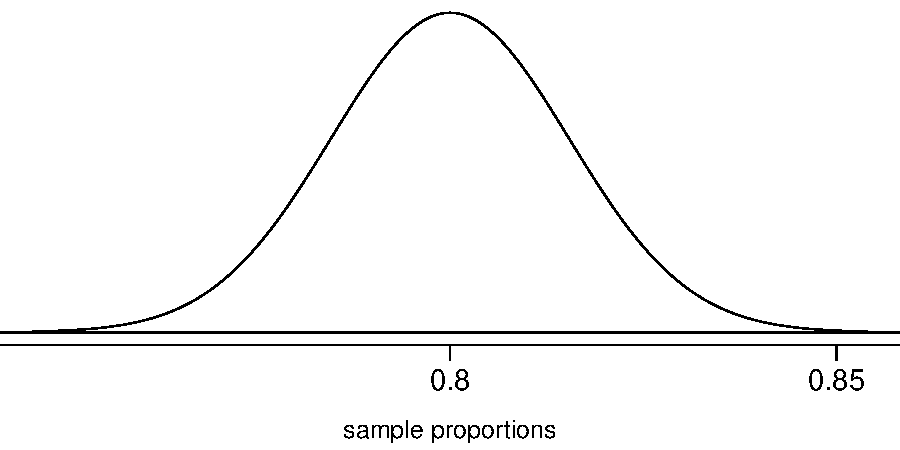
\includegraphics[width=\textwidth]{6-1_single_prop/figures/expdesgn_norm}
\end{center}
}
p値が低いため、$H_0$を棄却します。このデータは、80\%以上のアメリカ人が実験計画について正しい直感を持つという説得力のある証拠を提供します。

\end{frame}

%%%%%%%%%%%%%%%%%%%%%%%%%%%%%%%%%%%

\subsection{まとめ}

%%%%%%%%%%%%%%%%%%%%%%%%%%%%%%%%%%%

\begin{frame}
\frametitle{}

\pq{2006年のギャラップ調査に回答した1,001人のアメリカ人のうち、11\%が宗教的な理由からハロウィンのお祝いに反対していると回答しました。95\%信頼水準で、この調査の誤差の範囲は$\pm 3\%$です。この研究結果に関するニュース記事には「10\%以上のアメリカ人が宗教的な理由からハロウィンのお祝いに反対している」と書かれています。95\%信頼水準で、このニュース記事の主張は正当化されますか？}

\begin{enumerate}[(a)]
\item はい
\solnMult{いいえ}
\item 判断できない
\end{enumerate}

\end{frame}

%%%%%%%%%%%%%%%%%%%%%%%%%%%%%%%%%%

\begin{frame}
\frametitle{まとめ - 1つの割合の推測}

\begin{itemize}

\item 母集団のパラメータ：$p$、点推定値：$\hat{p}$

\item 条件：
\begin{itemize}
\item 独立性 \\
- 無作為標本かつ10\%条件
\item 少なくとも10の成功と失敗\\ - 満たさない場合 $\rightarrow$ 無作為化
\end{itemize}

\item 標準誤差：$SE = \sqrt{ \frac{p(1-p)}{n} }$
\begin{itemize}
\item CIの場合：$\hat{p}$を使用
\item HTの場合：$p_0$を使用
\end{itemize}

\end{itemize}

\end{frame}

%%%%%%%%%%%%%%%%%%%%%%%%%%%%%%%%%%%%

\section{2つの割合の差}

%%%%%%%%%%%%%%%%%%%%%%%%%%%%%%%%%%%%

\begin{frame}
\frametitle{北極の氷冠の融解}

\pq{科学者たちは、地球温暖化が今後100年以内に極地域に大きな影響を与える可能性があると予測しています。その一つとして、北極の氷冠が完全に融解する可能性があります。もしそれが実際に起きた場合、あなたはどの程度気になりますか？非常に気になる、ある程度気になる、少し気になる、まったく気にならない？}

\begin{enumerate}[(a)]
\item 非常に気になる
\item ある程度気になる
\item 少し気になる
\item まったく気にならない
\end{enumerate}

\end{frame}

%%%%%%%%%%%%%%%%%%%%%%%%%%%%%%%%%%%

\begin{frame}
\frametitle{GSSの結果}

GSSは同じ質問を行っており、以下は2010年のGSS調査およびデューク大学の入門統計学の学生グループからの回答の分布です：\\

\begin{center}
\begin{tabular}{l r r}
\hline
				& GSS	& デューク大 \\
\hline
非常に気になる		& 454	& 69 \\
ある程度気になる		& 124 	& 30\\
少し気になる		& 52 		& 4\\
まったく気にならない	& 50 		& 2 \\
\hline
合計				& 680 	& 105\\
\hline
\end{tabular}
\end{center}

\end{frame}

%%%%%%%%%%%%%%%%%%%%%%%%%%%%%%%%%%

\begin{frame}
\frametitle{母数（パラメータ）と点推定値}

\begin{itemize}

\item \hl{関心のある母数（パラメータ）：}\orange{全}デューク大学生と\orange{全}アメリカ人のうち、北極の氷冠の完全融解によって非常に気になると答える割合の差。
\[ \mathhl{ p_{デューク} - p_{米国} }\]

\item \hl{点推定値：}\orange{標本抽出された}デューク大学生と\orange{標本抽出された}アメリカ人のうち、北極の氷冠の完全融解によって非常に気になると答える割合の差。
\[ \mathhl{ \hat{p}_{デューク} - \hat{p}_{米国} }\]

\end{itemize}

\end{frame}

%%%%%%%%%%%%%%%%%%%%%%%%%%%%%%%%%%%

\begin{frame}
\frametitle{割合を比較するための推測}

\begin{itemize}

\item 詳細は以前と同じです…

\item CI：\textcolor{orange}{$点推定値 \pm 誤差の範囲$}

\item HT：\textcolor{orange}{$Z = \frac{点推定値 - 帰無値}{SE}$}を使って適切なp値を求めます。

\item 点推定値の適切な標準誤差（$SE_{ \hat{p}_{デューク} - \hat{p}_{米国}}$）が唯一の新しい概念です。

\end{itemize}

\formula{2つの標本割合の差の標準誤差}
{
\[ SE_{(\hat{p}_1 - \hat{p}_2)} = \sqrt{ \frac{p_1(1-p_1)}{n_1} + \frac{p_2(1-p_2)}{n_2} } \]
}

\end{frame}

%%%%%%%%%%%%%%%%%%%%%%%%%%%%%%%%%%%%%

\subsection{割合の差の信頼区間}

%%%%%%%%%%%%%%%%%%%%%%%%%%%%%%%%%%%%%

\begin{frame}
\frametitle{割合の差のCIの条件}

\begin{enumerate}

\item \hl{グループ内の独立性：}
\begin{itemize}
\item 米国グループは無作為に標本抽出されており、デューク大学グループも無作為標本を代表していると仮定します。
\item 105 $<$ 全デューク大学生の10\%、680 $<$ 全アメリカ人の10\%です。
\end{itemize}
標本内のデューク大学生の態度は互いに独立しており、標本内の米国住民の態度も互いに独立していると仮定できます。

\item \hl{グループ間の独立性：}
標本抽出されたデューク大学生と米国住民は互いに独立しています。

\item \hl{成功・失敗条件：}\\
2つのグループで少なくとも10の観測された成功と10の観測された失敗があること。

\end{enumerate}

\end{frame}

%%%%%%%%%%%%%%%%%%%%%%%%%%%%%%%%%%%%%

\begin{frame}
\frametitle{}

\dq{北極の氷冠の融解によって非常に気になると答えるデューク大学生とアメリカ人の割合の差\orange{($p_{デューク} - p_{米国}$)}について、95\%信頼区間を構築してください。}

{\footnotesize
\begin{center}
\begin{tabular}{l | c c}
データ			& デューク大	& 米国 \\
\hline
非常に気になる	& 69			& 454 \\
それ以外		& 36			& 226 \\
\hline
合計			& 105		& 680 \\
\hline
$\hat{p}$		& 0.657		& 0.668
\end{tabular}
\end{center}
}

\soln{
\begin{eqnarray*}
&& (\hat{p}_{D} - \hat{p}_{US}) \pm z^\star \times \sqrt{ \tfrac{ \hat{p}_{D} (1 - \hat{p}_{D})}{n_{D} } + \tfrac{ \hat{p}_{US} (1 -  \hat{p}_{US})}{n_{US} } }  \\
&=& (0.657 - 0.668) \pm 1.96 \times \sqrt{ \tfrac{0.657 \times 0.343}{105} + \tfrac{0.668 \times 0.332}{680} } \\
&=& -0.011 \pm 1.96 \times 0.0497 \\
&=& -0.011 \pm 0.097 \\
&=& (-0.108, 0.086)
\end{eqnarray*}
}


\end{frame}

%%%%%%%%%%%%%%%%%%%%%%%%%%%%%%%%%%%%%

\subsection{割合を比較するための仮説検定}

%%%%%%%%%%%%%%%%%%%%%%%%%%%%%%%%%%%%%

\begin{frame}

\pq{北極の氷冠の融解によって非常に気になると答えるデューク大学生全体の割合が、同様に答えるアメリカ人全体の割合と異なるかどうかを検定するための正しい仮説の組み合わせはどれですか？}

\begin{enumerate}[(a)]
\solnMult{ $H_0:  p_{デューク} = p_{米国}$ \\
$H_A:  p_{デューク} \ne p_{米国}$ }
\item $H_0:  \hat{p}_{デューク} = \hat{p}_{米国}$ \\
$H_A:  \hat{p}_{デューク} \ne \hat{p}_{米国}$
\solnMult{ $H_0:  p_{デューク} - p_{米国} = 0$ \\
$H_A:  p_{デューク} - p_{米国} \ne 0$ }
\item $H_0:  p_{デューク} = p_{米国}$ \\
$H_A:  p_{デューク} < p_{米国}$
\end{enumerate}

\soln{
\orange{(a)と(c)の両方が正しいです。}
}

\end{frame}

%%%%%%%%%%%%%%%%%%%%%%%%%%%%%%%%%%

\begin{frame}
\frametitle{1つの割合の検定への振り返り}

\begin{itemize}

\item 母集団の割合の信頼区間を構築する際は、\orange{観測された}成功数と失敗数が少なくとも10であるか確認します。
\[ n\hat{p} \ge 10 \qquad \qquad n(1-\hat{p}) \ge 10 \]

\item 母集団の割合の仮説検定を行う際は、\orange{期待される}成功数と失敗数が少なくとも10であるか確認します。
\[ np_0 \ge 10 \qquad \qquad n(1-p_0) \ge 10 \]

\end{itemize}

\end{frame}

%%%%%%%%%%%%%%%%%%%%%%%%%%%%%%%%%%%

\begin{frame}
\frametitle{割合のプールされた推定値}

\begin{itemize}

\item $H_0: p_1 = p_2$の場合に2つの割合を比較する際、各標本の\orange{期待される}成功数と失敗数を計算するために使える与えられた帰無値がありません。

\item そのため、まず2つのグループに共通の（\hl{プールされた}）割合を求め、それを分析に使用する必要があります。

\item これは単純に、観測総数のうちの成功の総数の割合を求めることを意味します。

\end{itemize}

$\:$ \\

\formula{割合のプールされた推定値}
{ \[ \hat{p} = \frac{\text{成功数}_1 + \text{成功数}_2}{n_1 + n_2} \] }

\end{frame}

%%%%%%%%%%%%%%%%%%%%%%%%%%%%%%%%%%%

\begin{frame}
\frametitle{}

\dq{北極の氷冠の融解によって非常に気になると答えるデューク大学生とアメリカ人の\underline{プールされた割合}を計算してください。プールされた推定値はどちらの標本割合（$\hat{p}_{デューク}$または$\hat{p}_{米国}$）に近いですか？なぜですか？}

{\footnotesize
\begin{center}
\begin{tabular}{l | c c}
データ			& デューク大	& 米国 \\
\hline
非常に気になる	& 69			& 454 \\
それ以外		& 36			& 226 \\
\hline
合計			& 105		& 680 \\
\hline
$\hat{p}$		& 0.657		& 0.668
\end{tabular}
\end{center}
}

\soln{
\begin{eqnarray*}
\hat{p} &=& \frac{\text{成功数}_1 + \text{成功数}_2}{n_1 + n_2} \\
&=& \frac{69+454}{105+680} = \frac{523}{785} = 0.666
\end{eqnarray*}
}

\end{frame}
%%%%%%%%%%%%%%%%%%%%%%%%%%%%%%%%%%%

\begin{frame}
\frametitle{}

\dq{これらのデータは、北極の氷冠の融解によって非常に気になると答えるデューク大学生全体の割合が、同様に答えるアメリカ人全体の割合と異なることを示唆していますか？検定統計量、p値を計算し、データの文脈で結論を解釈してください。}

{\footnotesize
\begin{center}
\begin{tabular}{l | c c}
データ			& デューク大	& 米国 \\
\hline
非常に気になる	& 69			& 454 \\
それ以外		& 36			& 226 \\
\hline
合計			& 105		& 680 \\
\hline
$\hat{p}$		& 0.657		& 0.668
\end{tabular}
\end{center}
}

\soln{
\begin{eqnarray*}
Z &=& \frac{(\hat{p}_{デューク} - \hat{p}_{米国})}{\sqrt{ \frac{ \hat{p} (1 - \hat{p})}{n_{デューク} } + \frac{ \hat{p} (1 -  \hat{p})}{n_{米国} } }} \\
&=& \frac{(0.657 - 0.668)}{\sqrt{ \frac{0.666 \times 0.334}{105} + \frac{0.666 \times 0.334}{680} }} = \frac{-0.011}{0.0495} = -0.22 \\
p\text{値} &=& 2 \times P(Z < -0.22) = 2 \times 0.41 = 0.82
\end{eqnarray*}
}

\end{frame}

%%%%%%%%%%%%%%%%%%%%%%%%%%%%%%%%%%%

\subsection{まとめ}

%%%%%%%%%%%%%%%%%%%%%%%%%%%%%%%%%%%

\begin{frame}
\frametitle{まとめ - 2つの割合の比較}

\begin{itemize}

\item 母集団のパラメータ：$(p_1 - p_2)$、点推定値：$(\hat{p}_1 - \hat{p}_2)$

\item 条件：
\begin{itemize}
\item グループ内の独立性 \\
- 両グループで無作為標本かつ10\%条件を満たす
\item グループ間の独立性
\item 各グループで少なくとも10の成功と失敗\\
- 満たさない場合 $\rightarrow$ 無作為化（6.4節）
\end{itemize}

\item $SE_{(\hat{p}_1 - \hat{p}_2)} = \sqrt{ \frac{p_1(1-p_1)}{n_1} + \frac{p_2(1-p_2)}{n_2} }$
\begin{itemize}
\item CIの場合：$\hat{p}_1$と$\hat{p}_2$を使用
\item HTの場合：
\begin{itemize}
\item $H_0: p_1 = p_2$の場合：$\hat{p}_{pool} = \frac{\text{成功}_1 + \text{成功}_2}{n_1 + n_2}$を使用
\item $H_0: p_1 - p_2 = $ \textit{（0以外の値）}の場合：$\hat{p}_1$と$\hat{p}_2$を使用 \\
- これはかなり稀
\end{itemize}
\end{itemize}

\end{itemize}

\end{frame}

%%%%%%%%%%%%%%%%%%%%%%%%%%%%%%%%%%%

\begin{frame}
\frametitle{参考 - 標準誤差の計算}

\begin{center}
\begin{tabular}{l | l | l}
			& 1標本					& 2標本 \\
\hline
& & \\
平均		& $SE = \frac{s}{\sqrt{n}}$			& $SE = \sqrt{ \frac{s_1^2}{n_1} + \frac{s_2^2}{n_2}}$ \\
& & \\
\hline
& & \\
割合		& $SE = \sqrt{ \frac{p(1-p)}{n} }$	& $SE = \sqrt{ \frac{p_1(1-p_1)}{n_1} + \frac{p_2(1-p_2)}{n_2} }$	 \\
& & \\
\end{tabular}
\end{center}

\begin{itemize}

\item 平均を扱う場合、$\sigma$が既知であることは非常に稀なので、通常$s$を使用します。

\item 割合を扱う場合、
\begin{itemize}
\item 仮説検定を行う場合、$p$は帰無仮説から来ます
\item 信頼区間を構築する場合、代わりに$\hat{p}$を使用します
\end{itemize}

\end{itemize}

\end{frame}

%%%%%%%%%%%%%%%%%%%%%%%%%%%%%%%%%%%%

\section{カイ二乗適合度検定}

%%%%%%%%%%%%%%%%%%%%%%%%%%%%%%%%%%%

\subsection{ウェルドンのサイコロ}

%%%%%%%%%%%%%%%%%%%%%%%%%%%%%%%%%%%

\begin{frame}
\frametitle{ウェルドンのサイコロ}

\twocol{0.75}{0.25}
{
\begin{itemize}

\item ウォルター・フランク・ラファエル・ウェルドン（1860--1906）は、イギリスの進化生物学者で、生物測定学の創設者の一人です。フランシス・ゴールトンおよびカール・ピアソンとともに、Biometrikaの共同創設編集者でした。

\item 1894年に、彼は12個のサイコロを26,306回振り、5か6が出た回数（成功とみなした）を記録しました。

\end{itemize}
}
{
\begin{center}
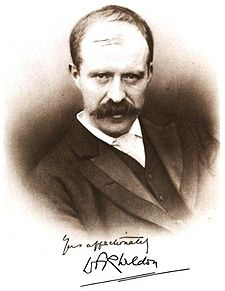
\includegraphics[width=\textwidth]{6-3_chisq_gof/figures/dice/weldon}
\end{center}
}
\begin{itemize}

\item 5か6が期待よりも頻繁に出ることが観察され、ピアソンはこれがサイコロの構造によるものだと仮説を立てました。安価なサイコロの多くは凹んだ点を持ち、反対の面の合計が7になるため、6の目のある面は1の目のある反対の面より軽くなります。

\end{itemize}

\end{frame}

%%%%%%%%%%%%%%%%%%%%%%%%%%%%%%%%%%%

\begin{frame}
\frametitle{ラビーのサイコロ}

\twocol{0.6}{0.4}
{
\begin{itemize}

\item 2009年、ザカライア・ラビー（シカゴ大学）は、手製のサイコロ投げ・点数カウント機械を使ってウェルドンの実験を再現しました。
\begin{center}
\webURL{http://www.youtube.com/watch?v=95EErdouO2w}
\end{center}

\item 転がして画像処理するのに約20秒かかりました。

\end{itemize}
}
{
\begin{center}
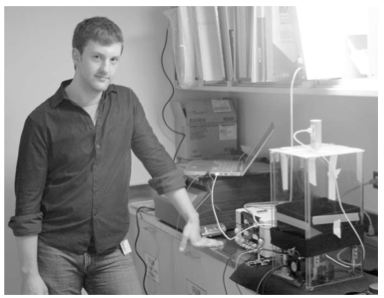
\includegraphics[width=\textwidth]{6-3_chisq_gof/figures/dice/labby}
\end{center}
}

\begin{itemize}

\item 1日あたり約150枚の画像を手動で処理する必要がありました。

\item このペースで、ウェルドンの実験は6日以上かけて再現されました。

\item 推薦読書：\webURL{http://galton.uchicago.edu/about/docs/labby09dice.pdf}

\end{itemize}

\end{frame}

%%%%%%%%%%%%%%%%%%%%%%%%%%%%%%%%%%%

\begin{frame}
\frametitle{ラビーのサイコロ（続き）}

\begin{itemize}

\item ラビーは実際には、ウェルドンが観察した現象（5と6の頻度が高い）を観察しませんでした。

\item 自動化によりラビーは1894年のウェルドンよりも多くのデータを収集でき、「成功」と「失敗」を記録する代わりに、各サイコロの個別の目の数を記録しました。

\end{itemize}

\begin{center}
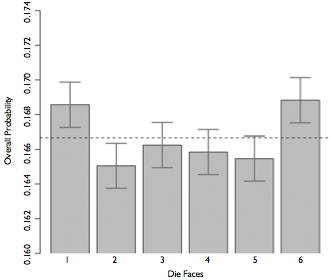
\includegraphics[width=0.5\textwidth]{6-3_chisq_gof/figures/dice/labbyPipCounts}
\end{center}

\end{frame}

%%%%%%%%%%%%%%%%%%%%%%%%%%%%%%%%%%%

\subsection*{一元表の検定統計量の作成}

%%%%%%%%%%%%%%%%%%%%%%%%%%%%%%%%%%%

\begin{frame}
\frametitle{期待度数}

\pq{ラビーは12個のサイコロを26,306回振りました。各面が等しい確率で出るとすれば、1、2、$\cdots$、6はそれぞれ何回出ることが期待されますか？}

\begin{enumerate}[(a)]
\item $\frac{1}{6}$
\item $\frac{12}{6}$
\item $\frac{26,306}{6}$
\solnMult{ $\frac{12 \times 26,306}{6}$ } \only<2->{\orange{$= 52,612$}}
\end{enumerate}

\end{frame}

%%%%%%%%%%%%%%%%%%%%%%%%%%%%%%%%%%%

\begin{frame}
\frametitle{ラビーの結果のまとめ}

以下の表は、ラビーの実験から得られた観測度数と期待度数を示しています。

{\small
\begin{center}
\renewcommand\arraystretch{1.2}
\begin{tabular}{c | c c}
結果	& 観測度数	& 期待度数 \\
\hline
1		& 53,222		& 52,612 \\
2		& 52,118		& 52,612 \\
3		& 52,465		& 52,612 \\
4		& 52,338		& 52,612 \\
5		& 52,244		& 52,612 \\
6		& 53,285		& 52,612 \\
\hline
合計		& 315,672		& 315,672
\end{tabular}
\end{center}
}

\dq{期待度数がすべての結果で同じなのに、観測度数が異なるのはなぜですか？一見して、観測度数と期待度数の間に不一致があるように見えますか？}

\end{frame}

%%%%%%%%%%%%%%%%%%%%%%%%%%%%%%%%%%%

\begin{frame}
\frametitle{仮説の設定}

\dq{これらのデータは、観測度数と期待度数の間の不一致の説得力のある証拠を提供しますか？}

\begin{itemize}
\item[$H_0$:] 観測度数と期待度数の間に不一致はありません。\hlGr{観測度数は期待度数と同じ分布に従います。}

\item[$H_A$:] 観測度数と期待度数の間に不一致があります。\hlGr{観測度数は期待度数と同じ分布に\orange{従いません}。}サイコロを振ったときに出る面にバイアスがあります。
\end{itemize}

\end{frame}

%%%%%%%%%%%%%%%%%%%%%%%%%%%%%%%%%%%

\begin{frame}
\frametitle{仮説の評価}

\begin{itemize}

\item これらの仮説を評価するために、観測度数が期待度数からどれだけ異なるかを定量化します。

\item 標本変動（偶然）のみによって期待される値から大きく逸脱している場合、対立仮説の強い証拠となります。

\item これは\hl{適合度}検定と呼ばれ、観測データが期待される分布にどの程度適合しているかを評価します。

\end{itemize}

\end{frame}

%%%%%%%%%%%%%%%%%%%%%%%%%%%%%%%%%%%

\subsection{カイ二乗統計量}

%%%%%%%%%%%%%%%%%%%%%%%%%%%%%%%%%%%

\begin{frame}
\frametitle{検定統計量の構造}

\begin{itemize}

\item 検定統計量の一般的な形は
\[ \frac{\text{点推定値} - \text{帰無値}}{\text{点推定値のSE}} \]

\item この構造は以下の2つに基づいています：
\begin{enumerate}
\item 帰無仮説が真の場合の期待値と点推定値の差を特定し、
\item その差を点推定値の標準誤差で標準化する。
\end{enumerate}

これらの2つの考え方が、度数データの適切な検定統計量の構築に役立ちます。

\end{itemize}

\end{frame}

%%%%%%%%%%%%%%%%%%%%%%%%%%%%%%%%%%%

\begin{frame}
\frametitle{カイ二乗統計量}

度数を扱い、観測度数が期待度数からどれだけ離れているかを調べる場合、\hl{カイ二乗（$\chi^2$）統計量}と呼ばれる新しい検定統計量を使用します。

$\:$ \\

\formula{$\chi^2$統計量}
{
\[\chi^2 = \sum_{i = 1}^k \frac{(O - E)^2}{E} \qquad \text{ここで$k$ = セルの総数} \]
}

\end{frame}

%%%%%%%%%%%%%%%%%%%%%%%%%%%%%%%%%%%

\begin{frame}
\frametitle{カイ二乗統計量の計算}

\begin{center}
\renewcommand\arraystretch{1.8}
\begin{tabular}{c | c c | c}
結果	& 観測度数	& 期待度数 	& $\frac{(O - E)^2}{E}$\\
\hline
1		& 53,222		& 52,612 		& $\frac{(53,222 - 52,612)^2}{52,612} = 7.07$ \\
2		& 52,118		& 52,612 		& $\frac{(52,118 - 52,612)^2}{52,612} = 4.64$ \\
3		& 52,465		& 52,612 		& $\frac{(52,465 - 52,612)^2}{52,612} = 0.41$ \\
4		& 52,338		& 52,612 		& $\frac{(52,338 - 52,612)^2}{52,612} = 1.43$\\
5		& 52,244		& 52,612 		& $\frac{(52,244 - 52,612)^2}{52,612} = 2.57$\\
6		& 53,285		& 52,612 		& $\frac{(53,285 - 52,612)^2}{52,612} = 8.61$\ \\
\hline
合計		& 315,672		& 315,672		& 24.73
\end{tabular}
\end{center}

\end{frame}

%%%%%%%%%%%%%%%%%%%%%%%%%%%%%%%%%%%

\begin{frame}
\frametitle{なぜ二乗するのか？}


観測された結果と期待された結果の差を二乗することは2つのことをします：
\begin{itemize}
\item 二乗された標準化された差はすべて正になります。
\item すでに異常に見えた差は、二乗後にさらに大きくなります。
\end{itemize}

\vspace{1cm}

\dq{以前にこのようなことを見たことがありますか？}

\end{frame}

%%%%%%%%%%%%%%%%%%%%%%%%%%%%%%%%%%%

\subsection{カイ二乗分布と面積の求め方}

%%%%%%%%%%%%%%%%%%%%%%%%%%%%%%%%%%%

\begin{frame}
\frametitle{カイ二乗分布}

\begin{itemize}

\item 計算した$\chi^2$統計量が異常に高いかどうかを判断するために、まずその分布を説明する必要があります。

\item カイ二乗分布は\hl{自由度（df）}と呼ばれる1つのパラメータのみを持ち、これが分布の形状、中心、広がりに影響します。\\

\end{itemize}

$\:$ \\

\Remember{これまでに3つの他の連続分布を見てきました：
\begin{itemize}
\item[-] 正規分布：平均と標準偏差の2つのパラメータを持つ単峰で対称な分布
\item[-] t分布：自由度の1つのパラメータを持つ単峰で対称な分布
\item[-] F分布：分子の自由度（グループ間分散）と分母の自由度（グループ内分散）の2つのパラメータを持つ単峰で右に歪んだ分布
\end{itemize}
}

\end{frame}

%%%%%%%%%%%%%%%%%%%%%%%%%%%%%%%%%%%

\begin{frame}
\frametitle{}

\pq{次のうち誤りはどれですか？}

\begin{center}
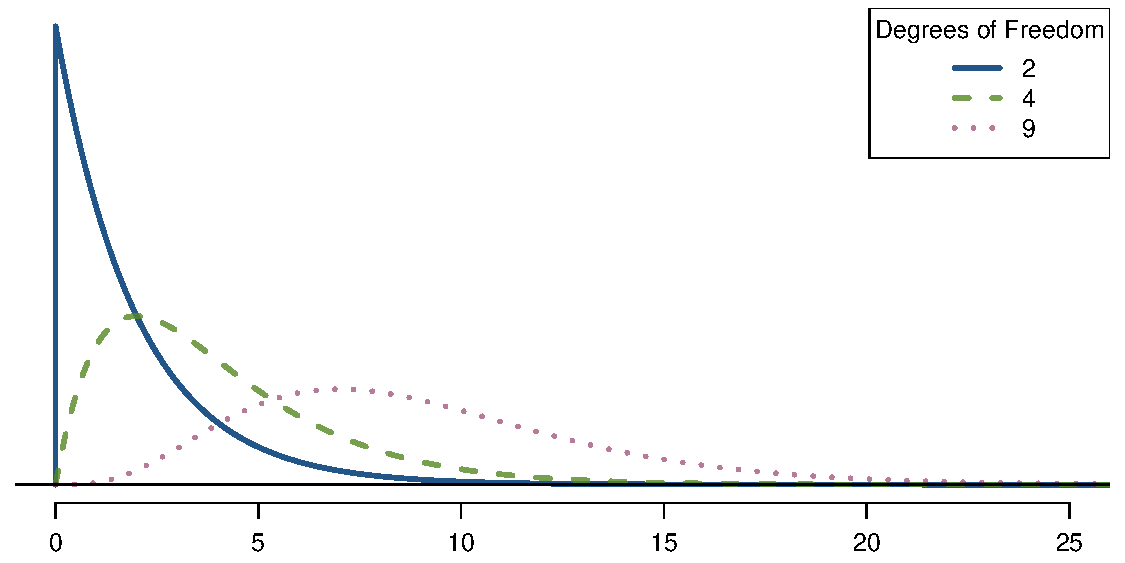
\includegraphics[width=0.7\textwidth]{6-3_chisq_gof/figures/chiSquareDistributionWithInceasingDF/chiSquareDistributionWithInceasingDF}
\end{center}

dfが増加するにつれて、
\begin{enumerate}[(a)]
\item $\chi^2$分布の中心も増加する
\item $\chi^2$分布のばらつきも増加する
\solnMult{$\chi^2$分布の形状がより歪んでくる（正規分布に近くなくなる）}
\end{enumerate}

\end{frame}

%%%%%%%%%%%%%%%%%%%%%%%%%%%%%%%%%%%

\begin{frame}[fragile]
\frametitle{カイ二乗曲線の下の面積を求める}

\begin{itemize}

\item p値 = カイ二乗分布の裾の面積（通常通り）

\item このためにテクノロジーやカイ二乗確率表を使用できます。

\end{itemize}

\end{frame}

%%%%%%%%%%%%%%%%%%%%%%%%%%%%%%%%%%%

\begin{frame}[fragile]
\frametitle{カイ二乗曲線の下の面積を求める（続き）}

\dq{$df = 6$の$\chi^2$曲線で、カットオフ値10より上の影付き部分の面積を推定してください。}

\begin{verbatim}

> pchisq(q = 10, df = 6, lower.tail = FALSE)

[1] 0.124652

\end{verbatim}

\end{frame}

%%%%%%%%%%%%%%%%%%%%%%%%%%%%%%%%%%%

\begin{frame}[fragile]
\frametitle{カイ二乗曲線の下の面積を求める（続き）}

\pq{$df = 9$の$\chi^2$曲線で、カットオフ値17より上の影付き部分の面積を推定してください。}

\twocol{0.6}{0.4}{
\begin{center}
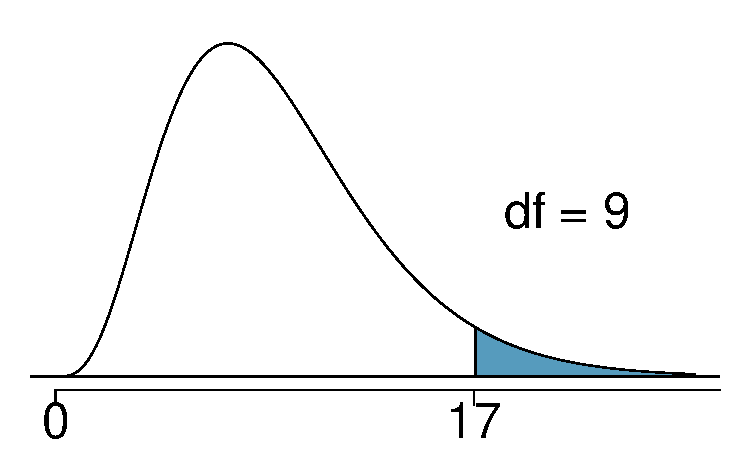
\includegraphics[width=0.67\textwidth]{6-3_chisq_gof/figures/above17WithDF9/above17WithDF9}
\end{center}
}
{
{\small
\begin{enumerate}[(a)]
\setlength{\itemsep}{0in}
\item 0.05
\item 0.02
\solnMult{0.02と0.05の間}
\item 0.05と0.1の間
\item 0.01と0.02の間
\end{enumerate}
}
}

\begin{verbatim}

> pchisq(q = 17, df = 9, lower.tail = FALSE)

[1] 0.04871598

\end{verbatim}

\end{frame}

%%%%%%%%%%%%%%%%%%%%%%%%%%%%%%%%%%%

\begin{frame}[fragile]
\frametitle{カイ二乗曲線の下の面積を求める（もう一問）}

\pq{$df = 10$の$\chi^2$曲線で、30より上の影付き部分の面積を推定してください。}

\twocol{0.6}{0.4}{
\begin{center}
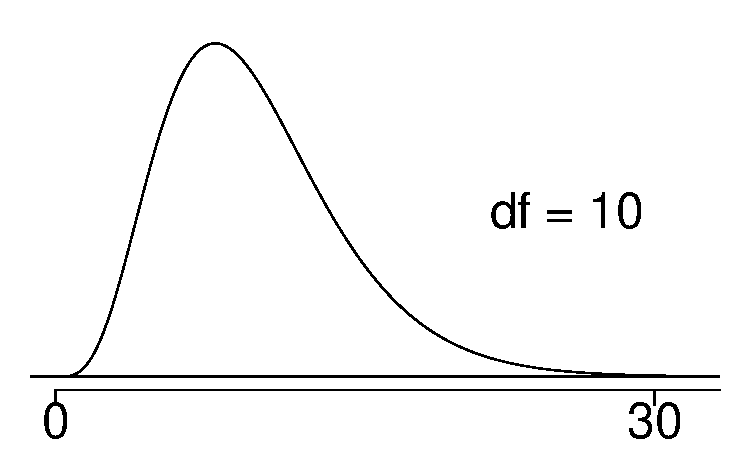
\includegraphics[width=0.67\textwidth]{6-3_chisq_gof/figures/above30WithDF10/above30WithDF10}
\end{center}
}
{
{\small
\begin{enumerate}[(a)]
\setlength{\itemsep}{0in}
\item 0.3より大きい
\item 0.005と0.001の間
\solnMult{0.001未満}
\item 0.001より大きい
\item この表では判断できない
\end{enumerate}
}
}

\begin{verbatim}

> pchisq(q = 30, df = 10, lower.tail = FALSE)

[1] 0.0008566412

\end{verbatim}

\end{frame}

%%%%%%%%%%%%%%%%%%%%%%%%%%%%%%%%%%%

\subsection{カイ二乗検定のp値の求め方}

%%%%%%%%%%%%%%%%%%%%%%%%%%%%%%%%%%%

\begin{frame}
\frametitle{ラビーのサイコロに戻ろう}

\begin{itemize}

\item 研究上の問いは：これらのデータは、観測度数と期待度数の間の不一致の説得力のある証拠を提供しますか？

\item 仮説は：
\begin{itemize}
\item[$H_0$:] 観測度数と期待度数の間に不一致はありません。観測度数は期待度数と同じ分布に従います。
\item[$H_A$:] 観測度数と期待度数の間に不一致があります。観測度数は期待度数と同じ分布に\orange{従いません}。サイコロを振ったときに出る面にバイアスがあります。
\end{itemize}

\item 検定統計量\orange{$\chi^2 = 24.67$}を計算しました。

\item $df$があれば、裾の面積（p値）を計算して仮説に関する決定を下すことができます。

\end{itemize}

\end{frame}

%%%%%%%%%%%%%%%%%%%%%%%%%%%%%%%%%%%

\begin{frame}
\frametitle{適合度検定の自由度}

\begin{itemize}

\item 観測データが期待される分布にどの程度適合しているかを評価する適合度検定では、自由度はセル数（$k$）から1を引いた値として計算されます。
\[ \mathhl{df = k - 1} \]

\item サイコロの結果では$k = 6$なので、
\[ df = 6 - 1 = 5 \]

\end{itemize}

\end{frame}

%%%%%%%%%%%%%%%%%%%%%%%%%%%%%%%%%%%

\begin{frame}
\frametitle{カイ二乗検定のp値の求め方}

カイ二乗検定の\hl{p値}は、\hl{計算された検定統計量より上の裾の面積}として定義されます。

\twocol{0.6}{0.4}{
\begin{center}
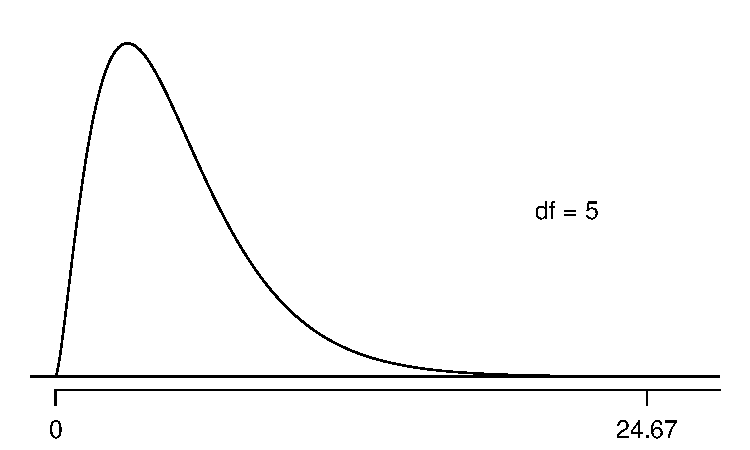
\includegraphics[width=0.67\textwidth]{6-3_chisq_gof/figures/above24Point67WithDF5/above24Point67WithDF5}
\end{center}
}
{
p値 = $P(\chi^2_{df = 5} > 24.67)$\\ は0.001未満
}

\end{frame}

%%%%%%%%%%%%%%%%%%%%%%%%%%%%%%%%%%%

\begin{frame}
\frametitle{仮説検定の結論}

\pq{p値が0.001未満と計算されました。有意水準5\%で、仮説検定の結論は何ですか？}

\begin{enumerate}[(a)]
\item $H_0$を棄却する：データはサイコロが公正であるという説得力のある証拠を提供します。
\solnMult{$H_0$を棄却する：データはサイコロに偏りがあるという説得力のある証拠を提供します。}
\item $H_0$を棄却しない：データはサイコロが公正であるという説得力のある証拠を提供します。
\item $H_0$を棄却しない：データはサイコロに偏りがあるという説得力のある証拠を提供します。
\end{enumerate}

\end{frame}

%%%%%%%%%%%%%%%%%%%%%%%%%%%%%%%%%%%

\begin{frame}
\frametitle{実は…}

\begin{itemize}

\item 1-6の軸は他の2つの軸（2-5と3-4）より一貫して短く、1の目と6の目のある面が他の面より大きいという仮説を支持しています。

\item 凹んだ点のために5と6がより頻繁に出るというピアソンの主張は、これらのデータによって支持されません。

\item カジノで使用されるサイコロはフラッシュフェースを持ち、点は周囲の素材と同じ密度のプラスチックで埋められ、精密にバランスが取られています。

\end{itemize}

\begin{center}
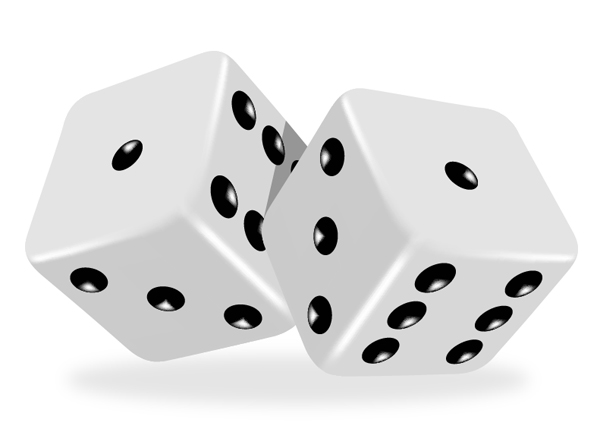
\includegraphics[width=0.3\textwidth]{6-3_chisq_gof/figures/dice/regular}
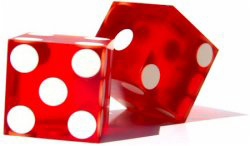
\includegraphics[width=0.3\textwidth]{6-3_chisq_gof/figures/dice/casino}
\end{center}


\end{frame}

%%%%%%%%%%%%%%%%%%%%%%%%%%%%%%%%%%%

\begin{frame}
\frametitle{まとめ：カイ二乗検定のp値}

\begin{itemize}

\item カイ二乗検定のp値は、計算された検定統計量の\hl{上の}裾の面積として定義されます。

\item 検定統計量は常に正であり、高い検定統計量ほど帰無仮説からの強い逸脱を意味するからです。

\end{itemize}

\begin{center}
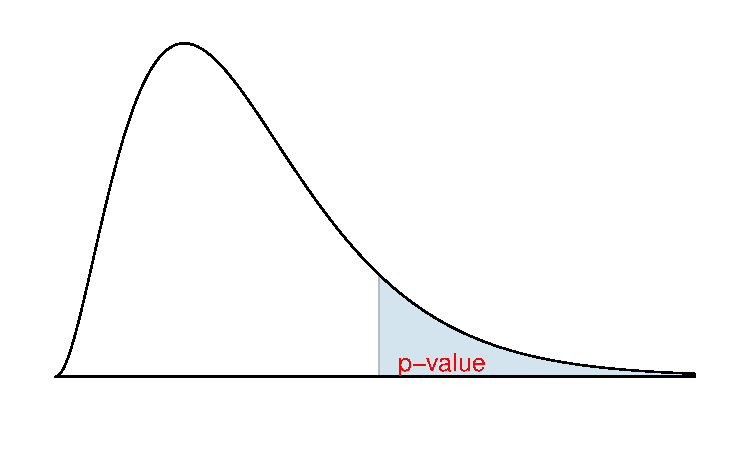
\includegraphics[width=0.7\textwidth]{6-3_chisq_gof/figures/genericChiSquare/genericChiSquare}
\end{center}

\end{frame}

%%%%%%%%%%%%%%%%%%%%%%%%%%%%%%%%%%%

\begin{frame}
\frametitle{カイ二乗検定の条件}

\begin{enumerate}

\item \hlGr{独立性：}表に度数を寄与する各ケースは、表の他のすべてのケースと独立していなければなりません。

\item \hlGr{標本サイズ：}各特定のシナリオ（すなわち、セル）は少なくとも5つの\orange{期待される}ケースがなければなりません。

\item \hlGr{$df > 1$：}自由度は1より大きくなければなりません。

\end{enumerate}

条件の確認を怠ると、意図せず検定の誤り率に影響を与える可能性があります。

\end{frame}

%%%%%%%%%%%%%%%%%%%%%%%%%%%%%%%%%%%

\subsection{2009年イラン選挙}

%%%%%%%%%%%%%%%%%%%%%%%%%%%%%%%%%%%

\begin{frame}
\frametitle{2009年イラン選挙}

\dq{2009年のイラン選挙では選挙不正が多く話題になりました。ここでは、選挙前に実施された世論調査のデータ（観測データ）と選挙で報告された得票率を比較して、両者が同じ分布に従うかどうかを確認します。}

\begin{center}
\begin{tabular}{l | r r}
					& \footnotesize{世論調査での観測} & \footnotesize{選挙での報告} \\
\footnotesize{候補者}	& \footnotesize{有権者数} & \footnotesize{得票率} \\
\hline
(1) アフマディネジャド	& 338	& 63.29\% \\
(2) ムサビ		& 136	& 34.10\% \\
(3) その他の候補者	& 30	& 2.61\% \\
\hline
合計			& 504	& 100\% \\
			& \hl{$\downarrow$}	& \hl{$\downarrow$}	\\
			& \hl{観測度数}	& \hl{期待される} \\
			& 			& \hl{分布}
\end{tabular}
\end{center}

\end{frame}

%%%%%%%%%%%%%%%%%%%%%%%%%%%%%%%%%%%

\begin{frame}
\frametitle{仮説}

\dq{報告された得票率と世論調査の分布が異なるかどうかを検定するための仮説は何ですか？}

\soln{
\begin{itemize}
\item[$H_0$:] 世論調査から観測された度数は、報告された得票率と同じ分布に従います。
\item[$H_A$:] 世論調査から観測された度数は、報告された得票率と同じ分布に従いません。
\end{itemize}
}

\end{frame}

%%%%%%%%%%%%%%%%%%%%%%%%%%%%%%%%%%%

\begin{frame}[shrink=10]
\frametitle{検定統計量の計算}

{\small
\begin{center}
\begin{tabular}{l | r r r}
				& \footnotesize{観測数} & \footnotesize{報告得票率}	& \footnotesize{期待数} \\
\footnotesize{候補者}	& \footnotesize{（世論調査）} & \footnotesize{（選挙）}		&  \footnotesize{（世論調査）} \\
\hline
\footnotesize{(1) アフマディネジャド}	& 338	& 63.29\% 	& 504 $\times$ 0.6329 = 319 \\
\footnotesize{(2) ムサビ}		& 136	& 34.10\%		& 504 $\times$ 0.3410 = 172 \\
\footnotesize{(3) その他の候補者}	& 30	& 2.61\% 		& 504 $\times$ 0.0261 = 13\\
\hline
合計			& 504	& 100\%		& 504
\end{tabular}
\end{center}
}

\begin{eqnarray*}
\tfrac{(338-319)^2}{319} &=& 1.13 \\
\tfrac{(136-172)^2}{172} &=& 7.53 \\
\tfrac{(30-13)^2}{13} &=& 22.23 \\
\chi^2_{\mathhl{df = 2}} &=& 30.89
\end{eqnarray*}


\end{frame}

%%%%%%%%%%%%%%%%%%%%%%%%%%%%%%%%%%%

\begin{frame}
\frametitle{結論}

\pq{これらの計算に基づいて、仮説検定の結論は何ですか？}

\begin{enumerate}[(a)]
\solnMult{p値が低く、$H_0$は棄却されます。世論調査から観測された度数は、報告された得票率と同じ分布に\underline{従いません}。}
\item p値が高く、$H_0$は棄却されません。世論調査から観測された度数は、報告された得票率と同じ分布に従います。
\item p値が低く、$H_0$は棄却されます。世論調査から観測された度数は、報告された得票率と同じ分布に従います。
\item p値が低く、$H_0$は棄却されません。世論調査から観測された度数は、報告された得票率と同じ分布に\underline{従いません}。
\end{enumerate}

\end{frame}

%%%%%%%%%%%%%%%%%%%%%%%%%%%%%%%%%%%%

\section{カイ二乗独立性検定}

%%%%%%%%%%%%%%%%%%%%%%%%%%%%%%%%%%%

\subsection{人気のある子供たち}

%%%%%%%%%%%%%%%%%%%%%%%%%%%%%%%%%%%

\begin{frame}[shrink=5]
\frametitle{人気のある子供たち}

\dq{\texttt{popular}データセットでは、4〜6年生が、良い成績・運動能力・人気のどれが最も重要かを尋ねられました。学年と最も重要な要因で分けた二元表を示します。目標が学年によって異なることを示す証拠はありますか？}

\twocol{0.5}{0.5}
{
\begin{center}
\begin{tabular}{rrrr}
  \hline
 & 成績 & 人気 & スポーツ \\
  \hline
$4$年生 &  63 &  31 &  25 \\
$5$年生 &  88 &  55 &  33 \\
$6$年生 &  96 &  55 &  32 \\
   \hline
\end{tabular}
\end{center}
}
{
\begin{center}
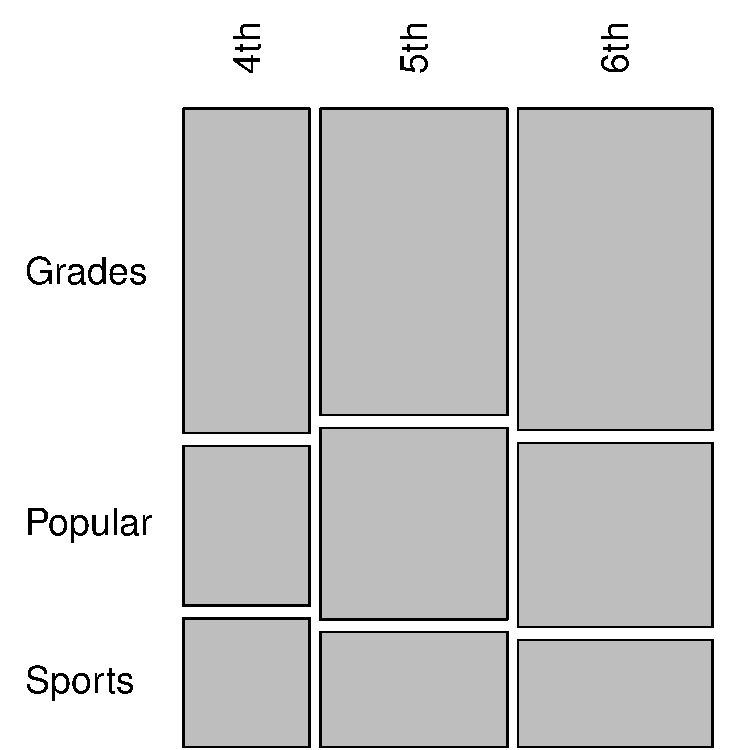
\includegraphics[width=0.75\textwidth]{6-4_chisq_indep/figures/popular/popular_mosaic}
\end{center}
}


\end{frame}

%%%%%%%%%%%%%%%%%%%%%%%%%%%%%%%%%%%

\begin{frame}
\frametitle{カイ二乗独立性検定}

\begin{itemize}
\item 仮説は：
\begin{itemize}
\item[$H_0$:] 学年と目標は独立しています。目標は学年によって異なりません。
\item[$H_A$:] 学年と目標は従属しています。目標は学年によって異なります。
\end{itemize}

\item 検定統計量は次のように計算されます：
\[ \chi^2_{df} = \sum_{i = 1}^{k} \frac{(O - E)^2}{E} \quad \text{ ここで } \quad df = (R - 1) \times (C - 1), \]
ここで$k$はセル数、$R$は行数、$C$は列数です。

\Note{一元表と二元表では$df$の計算が異なります。}

\item p値は$\chi^2_{df}$曲線の、計算された検定統計量より上の面積です。

\end{itemize}


\end{frame}

%%%%%%%%%%%%%%%%%%%%%%%%%%%%%%%%%%%

\subsection{二元表の期待度数}

%%%%%%%%%%%%%%%%%%%%%%%%%%%%%%%%%%%

\begin{frame}
\frametitle{二元表の期待度数}

\formula{二元表の期待度数}
{
\[ \text{期待度数} = \frac{(\text{行合計}) \times (\text{列合計})}{\text{表の合計}} \]
}

{\small
\begin{center}
\begin{tabular}{rrrr|r}
  \hline
 & 成績 & 人気 & スポーツ	& 合計 \\
  \hline
$4$年生 &  \orange{63} &  \green{31} &  25 	&119 \\
$5$年生 &  88 &  55 &  33	& 176 \\
$6$年生&  96 &  55 &  32	& 183 \\
   \hline
合計	& 247	& 141	& 90	& 478 \\
\end{tabular}
\end{center}
}

\[ \orange{$E_{\text{行1,列1}} = \frac{119 \times 247}{478} = 61$} \qquad
 \green{$E_{\text{行1,列2}} = \frac{119 \times 141}{478} = 35$} \]

\end{frame}

%%%%%%%%%%%%%%%%%%%%%%%%%%%%%%%%%%%

\begin{frame}
\frametitle{二元表の期待度数}

\pq{ハイライトされたセルの期待度数は何ですか？}

{\small
\begin{center}
\begin{tabular}{rrrr|r}
  \hline
 & 成績 & 人気 & スポーツ	& 合計 \\
  \hline
$4$年生 &  63 &  31 &  25 	&119 \\
$5$年生 &  88 &  \orange{55} &  33	& 176 \\
$6$年生 &  96 &  55 &  32	& 183 \\
   \hline
合計	& 247	& 141	& 90	& 478 \\
\end{tabular}
\end{center}
}

\twocol{0.2}{0.8}
{
\begin{enumerate}[(a)]
\solnMult{$\frac{176 \times 141}{478}$}
\item $\frac{119 \times 141}{478}$
\item $\frac{176 \times 247}{478}$
\item $\frac{176 \times 478}{478}$
\end{enumerate}
}
{
\soln{
\orange{$\rightarrow$ 52\\
{\small 期待より多くの5年生が \\
人気を目標としている}}
\vspace{0.75cm}
}
}

\end{frame}

%%%%%%%%%%%%%%%%%%%%%%%%%%%%%%%%%%%

\begin{frame}
\frametitle{二元表での検定統計量の計算}

期待度数は観測度数の隣に\ex{青色}で示されています。
\begin{center}
\begin{tabular}{rrrr|r}
  \hline
 & 成績 & 人気 & スポーツ	& 合計 \\
  \hline
$4$年生 	&  63 \ex{61} &  31 \ex{35} &  25 \ex{23}	&119 \\
$5$年生 	&  88 \ex{91} &  55 \ex{52} &  33 \ex{33}	& 176 \\
$6$年生	&  96 \ex{95} &  55 \ex{54} &  32 \ex{34}	& 183 \\
   \hline
合計	& 247	& 141	& 90	& 478 \\
\end{tabular}
\end{center}

\vspace{0.5cm}

\begin{eqnarray*}
\chi^2 &=& \sum \tfrac{(63-61)^2}{61} + \tfrac{(31-35)^2}{35} + \cdots + \tfrac{(32-34)^2}{34} = 1.3121 \\
df &=& (R - 1) \times (C - 1) = (3-1) \times (3-1) = 4
\end{eqnarray*}

\end{frame}

%%%%%%%%%%%%%%%%%%%%%%%%%%%%%%%%%%%

\subsection{結果}

%%%%%%%%%%%%%%%%%%%%%%%%%%%%%%%%%%%

\begin{frame}
\frametitle{p値の計算}

\pq{この仮説検定の正しいp値はどれですか？
\[ \chi^2 = 1.3121 \qquad df = 4 \]
}

\twocol{0.6}{0.4}{
\begin{center}
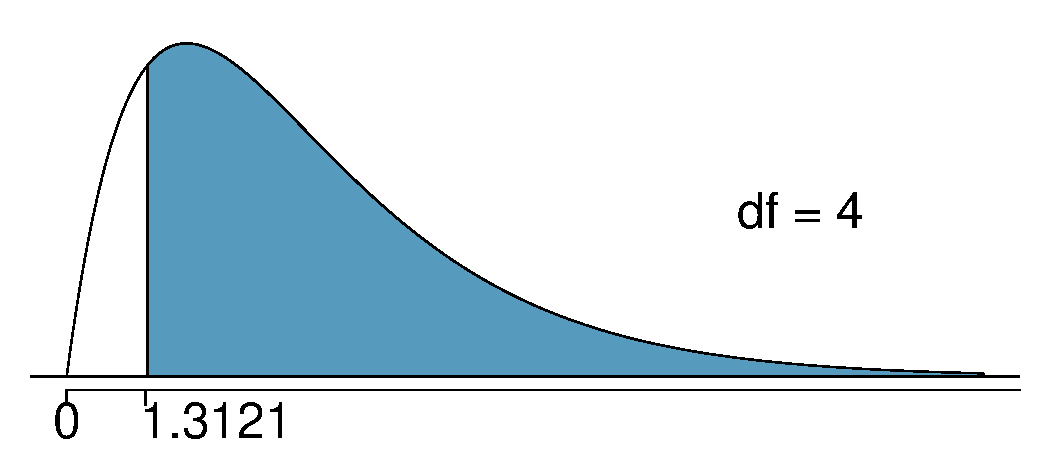
\includegraphics[width=0.67\textwidth]{6-4_chisq_indep/figures/popular/popular}
\end{center}
}
{
{\small
\begin{enumerate}[(a)]
\setlength{\itemsep}{0in}
\solnMult{ 0.3より大きい}
\item 0.3と0.2の間
\item 0.2と0.1の間
\item 0.1と0.05の間
\item 0.001未満
\end{enumerate}
}
}

\end{frame}

%%%%%%%%%%%%%%%%%%%%%%%%%%%%%%%%%%%

\begin{frame}
\frametitle{結論}

\dq{これらのデータは、目標が学年によって異なることを示す証拠を提供しますか？}

\begin{itemize}

\item[$H_0$:] 学年と目標は独立しています。目標は学年によって異なりません。

\item[$H_A$:] 学年と目標は従属しています。目標は学年によって異なります。\\

\end{itemize}

$\:$ \\

\soln{p値が高いため、$H_0$を棄却しません。データは学年と目標が従属しているという説得力のある証拠を提供しません。目標は学年によって異ならないようです。
}

\end{frame}



%%%%%%%%%%%%%%%%%%%%%%%%%%%%%%%%%%%%
% ドキュメント終了
%%%%%%%%%%%%%%%%%%%%%%%%%%%%%%%%%%%%

\end{document}
